\documentclass[12pt]{article}
\usepackage[utf8]{inputenc}
\usepackage[greek,english]{babel}
\usepackage{alphabeta}
\usepackage{fancyhdr}
\usepackage{listings}
\usepackage{mathtools}
\usepackage{xcolor}
\usepackage{float}
\usepackage{tabularx}
\usepackage[margin=0.5in]{geometry}
\usepackage[backend=bibtex]{biblatex}
\usepackage{hyperref}
\hypersetup{
	colorlinks=true, %set true if you want colored links
	linktoc=all,     %set to all if you want both sections and subsections linked
	linkcolor=black,  %choose some color if you want links to stand out
}
\title{Εργασία Τεχνολογίας Λογισμικού -- Μέρος 1ο}
\author{Αντώνης Θωμάκος - 18390037 \\
Χρήστος Μαργιώλης - 19390133 \\
Στέφανος Στράους - 19390221}
\date{Μάρτιος 2022}

\begin{document}

\begin{titlepage}
        \maketitle
        \begin{figure}[t!]
        \begin{center}
        
\includegraphics[scale=1.0]{./res/uniwa-logo.pdf} \\
        \Large
        \textbf{Πανεπιστήμιο Δυτικής Αττικής} \\
        \large
        Τμήμα Μηχανικών Πληροφορικής και Ηλεκτρονικών Υπολογιστών
        \end{center}
        \end{figure}
\end{titlepage}

\renewcommand{\contentsname}{Περιεχόμενα}
\tableofcontents
\pagebreak

\section{Σκοπός του Π.Σ διαχείρισης αεροδρομίου}

Το εξής πληροφοριακό σύστημα έχει σκοπό την ολική διαχείριση κάθε πτυχής του
αεροδρομίου. Συγκεκριμένα, θα διαχειρίζεται τις κρατήσεις θέσεων από επιβάτες,
δηλαδή το ταμείο από το οποίο οι πελάτες θα μπορούν να κλείσουν θέση σε κάποια
πτήση. Στην συνέχεια, το σύστημα θα πρέπει να ελέγχει την εγκυρότητα κάθε
εισιτηρίου λίγο πριν την επιβίβαση του πελάτη στο αεροπλάνο (check in) και να
ενημερώνει το σύστημα κατάλληλα για την πληρότητα του αεροπλάνου. Είναι επίσης
απαραίτητες οι πληροφορίες για τις πτήσεις, συγκεκριμένα στις αναχωρήσεις και
αφίξεις πτήσεων. Παρέχει επίκαιρες πληροφορίες για καθυστερήσεις ακυρώσεις
πτήσεων κ.α. Επιπροσθέτως, για να διασφαλιστεί η ασφάλεια της κάθε πτήσης
ελέγχονται οι αποσκευές των επιβατών για τυχόν απαγορευμένες ουσίες καθώς και
για όπλα ή εκρηκτικές ύλες. Αυτά τα ευρήματα καταγράφονται σε βάση δεδομένων
του συστήματος. Σε κάθε πτήση, είναι σημαντικό οι αποσκευές των επιβατών, καθώς
και διάφορα άλλα τυχόν πακέτα να καταγράφονται και να είναι δηλωμένα στο
σύστημα με σκοπό να αποφυγει η απώλεια τους. Δεν γίνεται να ξεχαστούν τα
αναλώσιμα πτήσης, κυρίως τα τρόφιμα που παρέχονται στο προσωπικό και στους
επιβάτες. Εξίσου σημαντική είναι η επιμελητεία των πόρων (logistics), δηλαδή ο
συνεχής εφοδιασμός των αεροπλάνων με καύσιμα, και η διατήρηση τους σε κατάσταση
κατάλληλη για πτήση από τους μηχανικούς. Το σύστημα αυτό πρέπει να είναι
διατεθειμένο να χειριστεί μεγάλο αριθμό υλών, καθώς και την ποσότητα τους ώστε
να υπάρχει πάντα έγκυρη εικόνα των διαθέσιμων επιπέδων καυσίμου, ανταλλακτικών
κτλ. Τέλος, ο πύργος ελέγχου πρέπει να δέχεται έγκαιρα όλες τις πληροφορίες
καιρού από μετεωρολογικούς σταθμούς, να έχει μια ολική εικόνα του αεροχώρου
μέσω διαφόρων radar, και να είναι γενικώς πάντα ενημερωμένοι οι υπάλληλοι που
δουλεύουν σε αυτόν.

\section{Χρήστες -- Actors}

\begin{itemize}
	\item Μηχανικοί εδάφους
	\begin{itemize}
		\item Χαρακτηριστικά: Είναι οι μηχανικοί που ελέγχουν και επισκευάζουν
			κάθε αεροσκάφος.
		\item Απαιτήσεις:
			\begin{itemize}
			\item Ειδοποιούνται από το σύστημα λίγο πριν την άφιξη του
				αεροπλάνου.
			\item Το σύστημα πρέπει να τους παρέχει πληροφορίες για την
				κατάσταση του αεροσκάφους λίγο πριν την άφιξή του.
			\end{itemize}
	\end{itemize}
	\item Προσωπικό ταμείου
	\begin{itemize}
		\item Χαρακτηριστικά: Παρέχουν βοήθεια στους επιβάτες.
		\item Απαιτήσεις: Να ελέγχουν τις κρατήσεις και να βοηθούν τους
			πελάτες κατά την διάρκεια της κράτησης του εισιτηρίου.
	\end{itemize}
	\item Προσωπικό ασφαλείας
	\begin{itemize}
		\item Χαρακτηριστικά: Βρίσκεται στο τερματικό (terminal) του
			αεροδρομίου.
		\item Απαιτήσεις: Ελέγχουν τα αποτελέσματα του συστήματος και
			σε περίπτωση εύρεσης επικίνδυνου αντικειμένου, απαγορεύουν
			στον επιβάτη να συνεχίσει προς το αεροπλάνο.
	\end{itemize}
	\item Προσωπικό εδάφους
	\begin{itemize}
		\item Χαρακτηριστικά: Πραγματοποιούν τους εφοδιασμούς του
			αεροπλάνου.
		\item Απαιτήσεις: Πρέπει να ειδοποιηθούν από το σύστημα για τυχόν
			ελλείψεις αναλώσιμων στο αεροσκάφος.
	\end{itemize}
	\item Επιβάτης
	\begin{itemize}
		\item Απαιτήσεις: Αλληλεπιδρά με το σύστημα κράτησης εισιτηρίων,
			καθώς και όλα τα συστήματα ελέγχου.
	\end{itemize}
\end{itemize}

\section{Λειτουργικές και μη απαιτήσεις}

Οι λειτουργικές απαιτήσεις του Π.Σ είναι αναλύει τα δεδομένα που δέχεται (π.χ
από τον πύργο ελέγχου, από το σύστημα κράτησης εισιτηρίων, κλπ) και το
προσωπικό που βασίζεται σε αυτές να ενημερώνεται έγκαιρα και να εξασφαλίζεται η
σωστή λειτουργία του αεροδρομίου.

Οι μη-λειτουργικές του Π.Σ περιλαμβάνουν την εξοικείωση του προσωπικού με τα
διάφορα υποσυστήματα που χρησιμοποιεί το κάθε τμήμα του αεροδρομίου, καθώς και
η αξιοπιστία που πρέπει να παρέχει γενικότερα το Π.Σ. Η αξιοπιστία
επιτυγχάνεται από το γεγονός ότι όλα τα υποσυστήματα μοιράζονται κοινές βάσεις
δεδομένων, με αποτέλεσμα να υπάρχει συγχρονισμός των δεδομένων.

\section{Περιπτώσεις χρήσης -- Use cases}

\subsection{Πίνακας ΠΧ}

\begin{center}
\begin{tabular}{|l|p{7cm}|p{7cm}|}
	\hline
	\textbf{Κωδικός} & \textbf{'Ονομα} & \textbf{Περιγραφή} \\
	\hline
	ΠΧ1 & Κρατήσεις εισιτηρίων/θέσεων (booking) &
	Το σύστημα δείχνει στον επιβάτη τις διαθέσιμες πτήσεις. Αφού ο επιβάτης
	κάνει την αγορά, το σύστημα τυπώνει το εισιτήριο και ενημερώνει την
	βάση δεδομένων αποθεμάτων εισιτηρίων και θέσεων που κρατάει το
	αεροδρόμιο. \\
	\hline
	ΠΧ2 & 'Ελεγχος εγκυρότητας εισιτηρίων (check in) &
	Πραγματοποιεί τον τελικό έλεγχο πριν την είσοδο του επιβάτη στο
	αεροπλάνο. \\
	\hline
	ΠΧ3 & Πληροφορίες πτήσης (αναχωρήσεις, αφίξεις, καθυστερήσεις,
	ακυρωμένες πτήσεις, …) & Ενημέρωση πινάκων αεροδρομίου (Flight
	Information Display System - FIDS) σχετικά με τις επερχόμενες
	αναχωρήσεις και αφίξεις, καθώς γεγονότα που μπορεί να τις επηρεάσουν
	(καιρικές συνθήκες, απρόοπτα συμβάντα, ...). \\
	\hline
	ΠΧ4 & 'Ελεγχος ασφαλείας πτήσης (safety checks) &
	Σαρώνει και κρίνει αν υπάρχουν επικίνδυνες ύλες στις αποσκευές με
	χρήση ανιχνευτή μετάλλων και καταγράφει τα ευρύματα σε βάση
	δεδομένων. \\
	\hline
	ΠΧ5 & Δρομολόγηση αποσκευών (cargo/luggage logistics) &
	Στέλνει τις αποσκευές στο κατάλληλο αμπάρι φορτίου κατά την αναχώρηση
	και στον κύλινδρο φορτίου κατά την άφιξη. \\
	\hline
	ΠΧ6 & 'Ελεγχος αναλώσιμων πτήσης (in-flight logistics) &
	Καταγράφει το αναλωσίμων (φαγητό, ποτά, μάσκες μίας χρήσης, σωσίβια,
	...) και ειδοποιεί το προσωπικό εδάφους σε περίπτωση ανεφοδιασμού. \\
	\hline
	ΠΧ7 & Τεχνικός έλεγχος αεροπλάνων και καυσίμων (maintenance, refuelling) &
	Καταγράφεται η μηχανική κατάσταση του αεροπλάνου και το απόθεμα του σε
	καύσιμο κατά την αναχώρηση και άφιξη. \\
	\hline
	ΠΧ8 & Air Traffic Control &
	Χειρίζεται τα δεδομένα που έχουν να κάνουν με τον πύργο ελέγχου, όπως
	να κρίνεται αν είναι δυνατή η κανονική λειτουργία των πτήσεων με βάση
	τις καιρικές συνθήκες που επικρατούν, τα ραντάρ του πύργου καθώς και
	πληροφορίες σχετικά με τρέχουσες πτήσεις. \\
	\hline
\end{tabular}
\end{center}

\subsection{Διαγράμματα Use Case}

\begin{figure}[H]
	\centering
	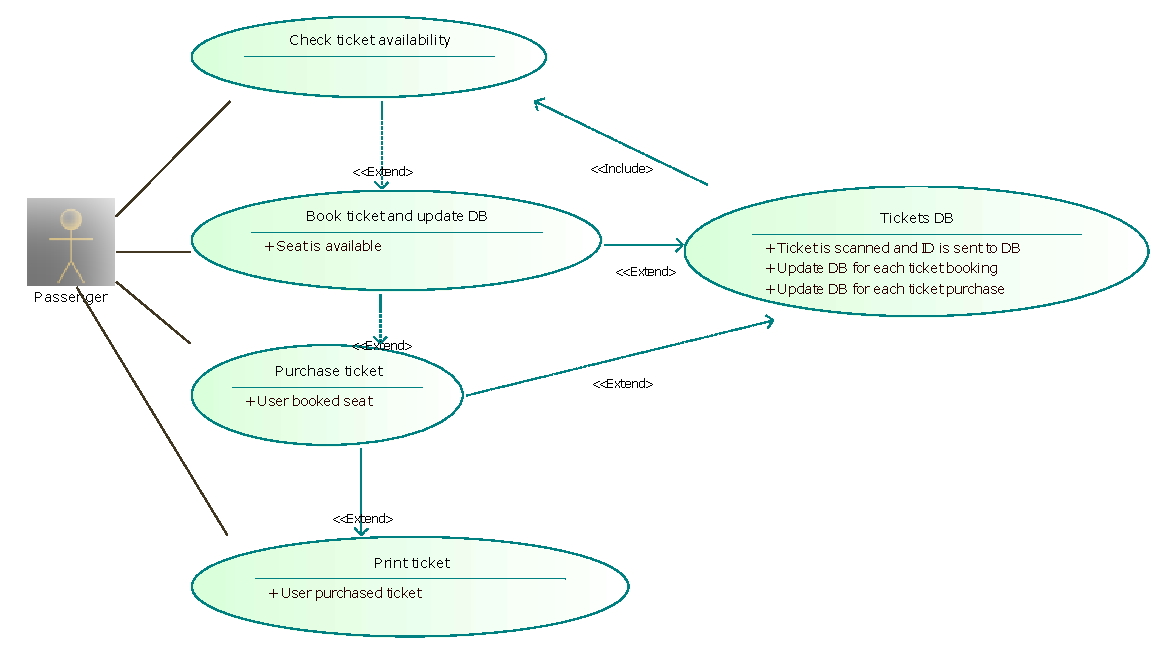
\includegraphics[width=\linewidth]{./res/uc1.pdf}
	\caption{Use Case 1 -- Κρατήση εισιτηρίων/θέσεων.}
\end{figure}

\begin{figure}[H]
	\centering
	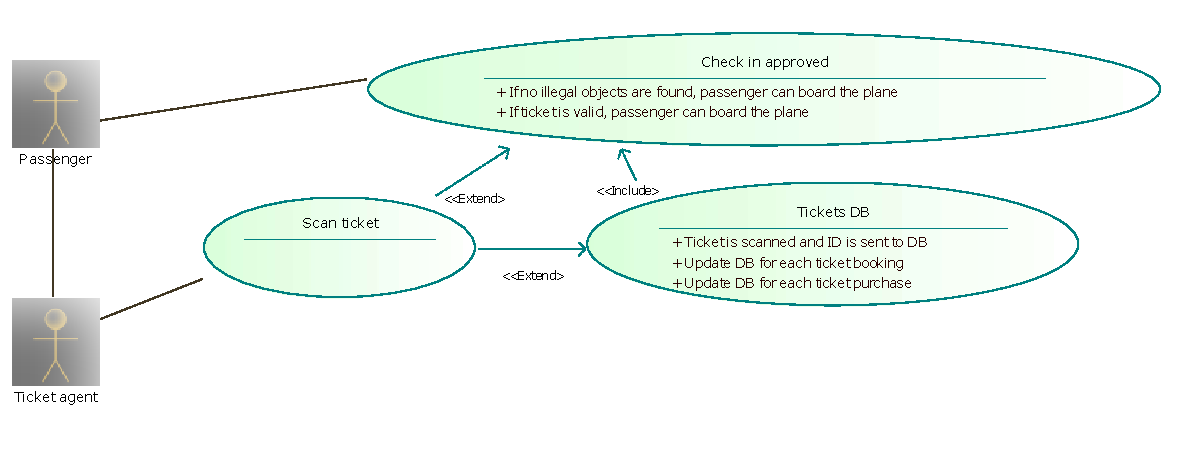
\includegraphics[width=\linewidth]{./res/uc2.pdf}
	\caption{Use Case 2 -- 'Ελεγχος εγκυρότητας εισιτηρίων (check in).}
\end{figure}

\begin{figure}[H]
	\centering
	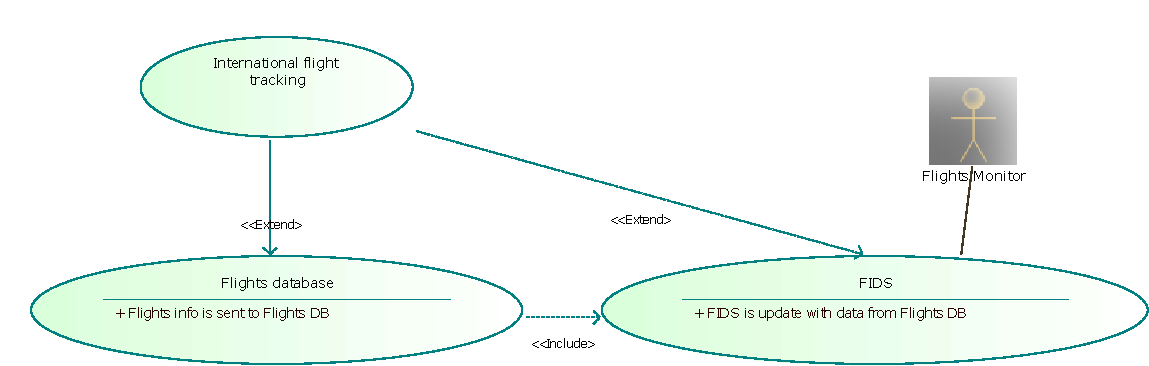
\includegraphics[width=\linewidth]{./res/uc3.pdf}
	\caption{Use Case 3 -- Πληροφορίες πτήσης.}
\end{figure}

\begin{figure}[H]
	\centering
	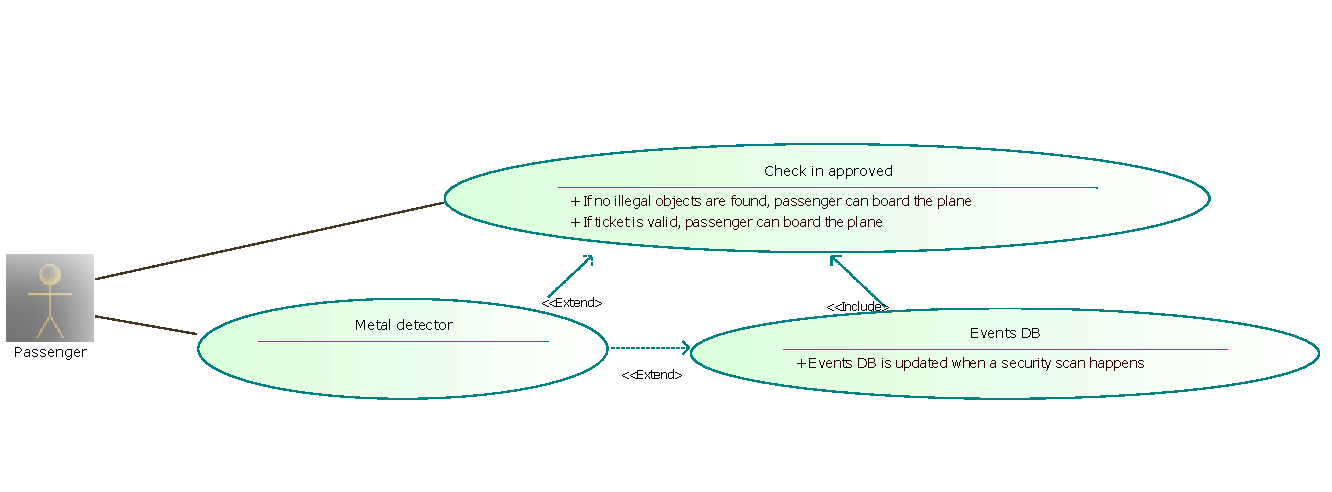
\includegraphics[width=\linewidth]{./res/uc4.pdf}
	\caption{Use Case 4 -- 'Ελεγχος ασφαλείας αποσεκυών.}
\end{figure}

\begin{figure}[H]
	\centering
	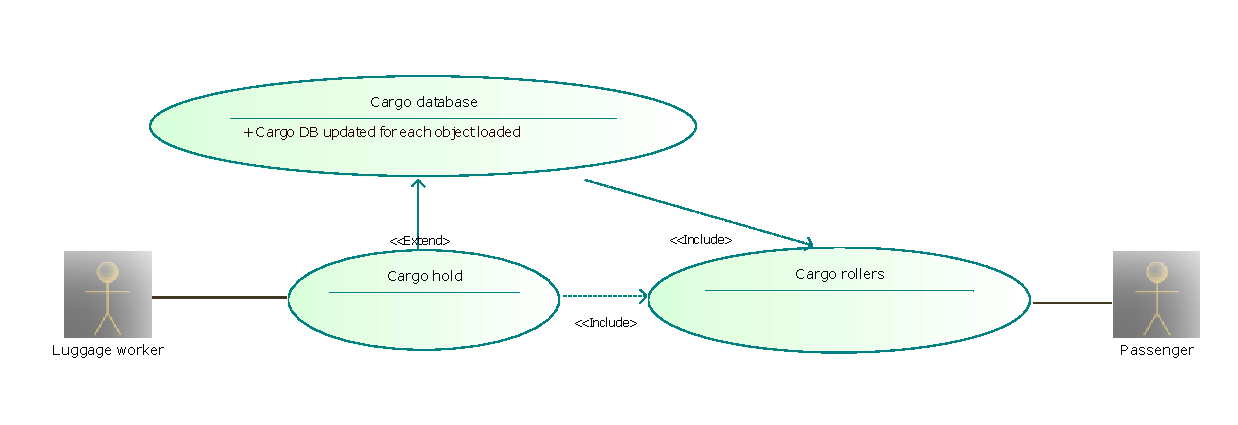
\includegraphics[width=\linewidth]{./res/uc5.pdf}
	\caption{Use Case 5 -- Δρομολόγηση αποσκευών.}
\end{figure}

\begin{figure}[H]
	\centering
	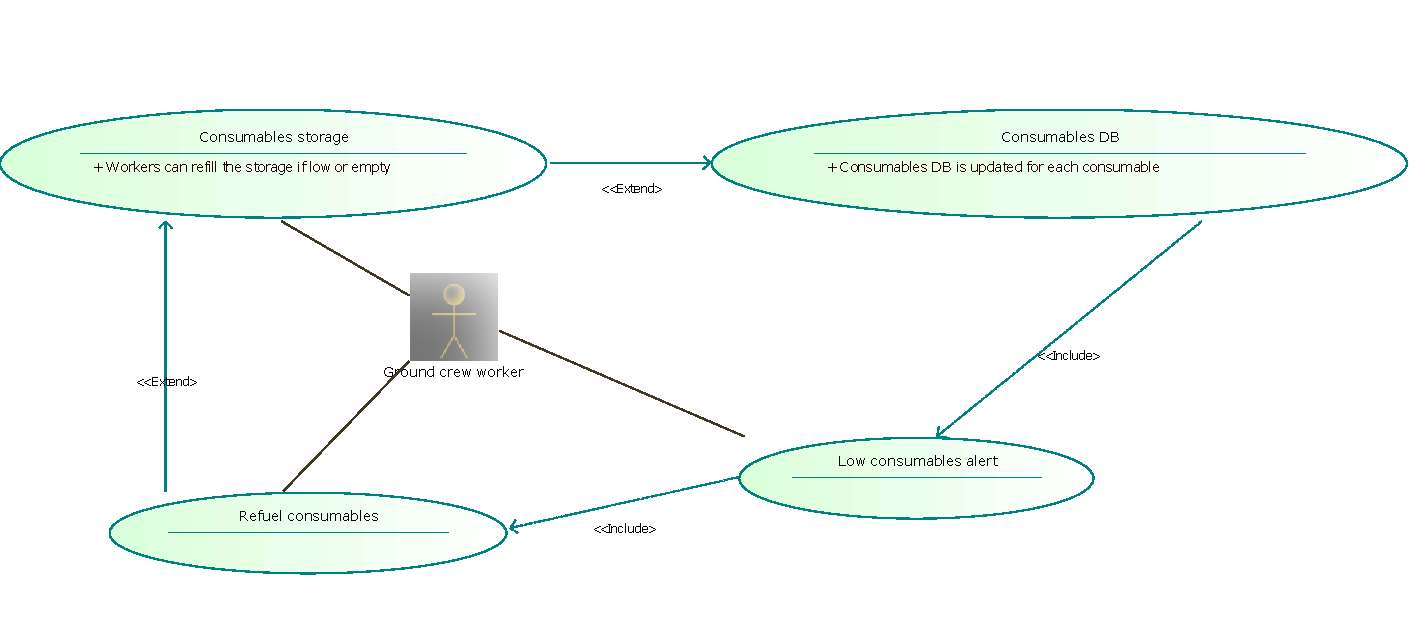
\includegraphics[width=\linewidth]{./res/uc6.pdf}
	\caption{Use Case 6 -- 'Ελεγχος καυσίμων και αναλώσιμων πτήσης.}
\end{figure}

\begin{figure}[H]
	\centering
	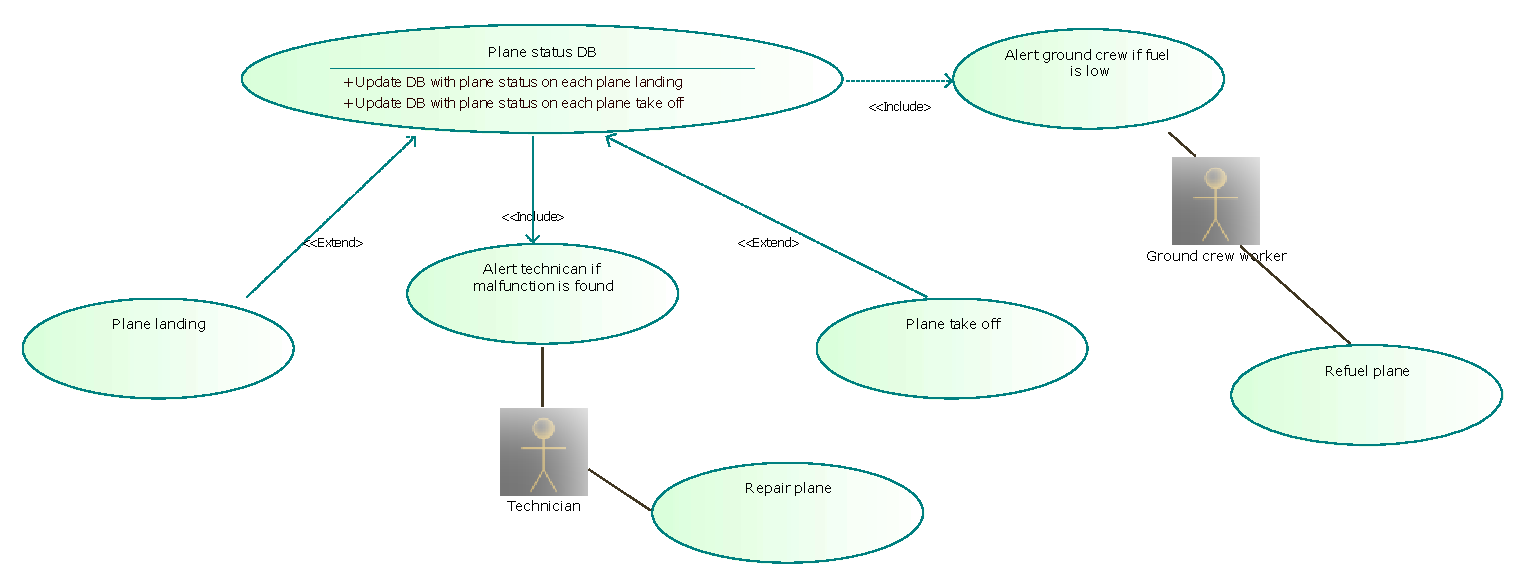
\includegraphics[width=\linewidth]{./res/uc7.pdf}
	\caption{Use Case 7 -- Τεχνικός έλεγχος αεροπλάνων.}
\end{figure}

\begin{figure}[H]
	\centering
	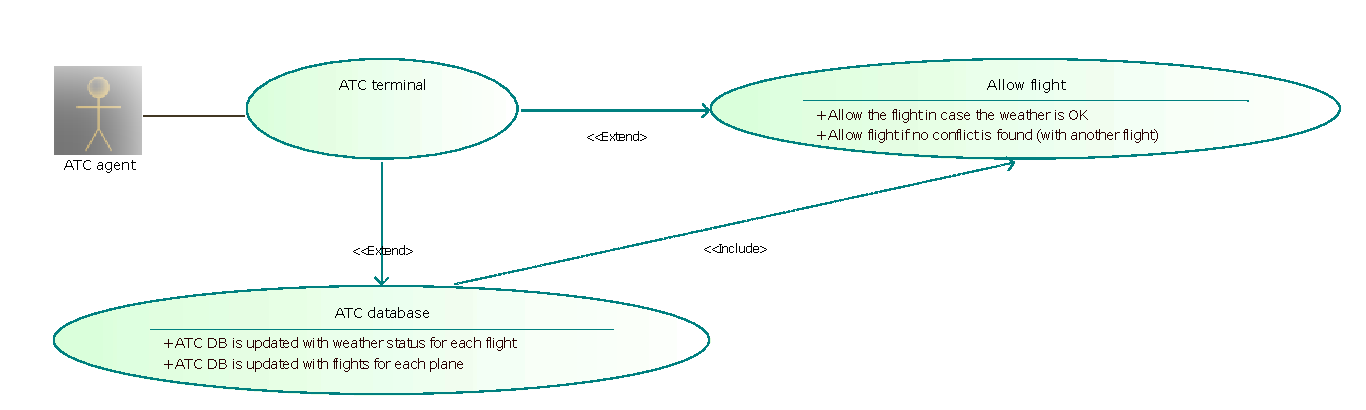
\includegraphics[width=\linewidth]{./res/uc8.pdf}
	\caption{Use Case 8 -- Λήψη μετεωρολογικής πρόγνωσης.}
\end{figure}

\pagebreak
\subsection{Πίνακας τεκμηρίωσης}

\subsubsection{Κρατήσεις εισιτηρίων}

\begin{center}
\begin{tabular}{|p{5cm}|p{12cm}|}
	\hline
	\textbf{Use Case} & Κρατήσεις εισιτηρίων (ημερομηνία, αριθμός πτήσης
	κτλ). \\
	\hline
	\textbf{Σύντομη περιγραφή} & Ο επιβάτης χρησιμοποιεί το σύστημα
	κράτησης, ορίζοντας σε αυτό στοιχεία για το εισιτήριο του όπως:
	\textit{ημερομηνία άφιξης}, \textit{ημερομηνία
	αναχώρησης}, \textit{αριθμός πτήσης},
	\textit{θέση}, \textit{αριθμός επιπλέον
	αποσκευών} κλπ. \\
	\hline
	\textbf{Actors} & Επιβάτης, Προσωπικό ταμείου (Ρεσεψιόν). \\
	\hline
	\textbf{Προαπαιτούμενα (Pre-conditions)} &
	\begin{itemize}
		\item Το σύστημα να λειτουργεί κανονικά.
		\item Το προσωπικό να κάνει την κράτηση του πελάτη.
	\end{itemize} \\
	\hline
	\textbf{Μετασυνθήκες (Post-conditions)} & Μετά την κράτηση, το
	πληροφοριακό σύστημα έχει δηλωμένα τα στοιχεία για την πτήση και ο
	πελάτης έχει εξασφαλίσει μια θέση σε αυτήν \\
	\hline
	\textbf{Κύρια ροή} &
	\begin{tabularx}{12cm}{X|X}
		\textbf{Tasks} & \textbf{Πληροφορία που απαιτείται/διαμοιράζεται} \\ 
		\hline
		Το use case ξεκινά με την εισαγωγή των στοιχείων του επιβάτη
		στο σύστημα δηλαδή των παραμέτρων του εισιτηρίου. &
		Ημερομηνία αναχώρησης, Ημερομηνία άφιξης, Αριθμός Θέσης,
		Αριθμός Πτήσης, Επιπλέον Αποσκευές, Αριθμός Εισιτηρίου. \\
		\hline
		Το σύστημα ελέγχει αν η θέση είναι διαθέσιμη. & \\
		\hline
		Το πληροφοριακό σύστημα αποκρίνεται αποθηκεύοντας τα δεδομένα
		στο σύστημα, ελέγχοντας τα ταυτόχρονα για την εγκυρότητα τους,
		όπου δίνεται ευκαιρία στον υπάλληλο να τα διορθώσει. & \\
		\hline
		Το σύστημα εκδίδει το εισιτήριο. & \\
	\end{tabularx} \\
\hline
	\textbf{Εναλλακτική ροή} &
	\begin{tabularx}{12cm}{X|X}
		\textbf{Tasks} & \textbf{Πληροφορία που απαιτείται/διαμοιράζεται} \\ 
		\hline
		Εναλλακτικά, αν η θέση δεν είναι διαθέσιμη, το σύστημα ενημερώνει τον υπάλληλο με κατάλληλο μύνημα. & \\
	\end{tabularx} \\
	\hline
\end{tabular}
\end{center}

\pagebreak
\subsubsection{'Ελεγχος Εγκυρότητας Εισιτηρίων (Check In)}

\begin{center}
\begin{tabular}{|p{5cm}|p{12cm}|}
	\hline
	\textbf{Use Case} & Check in εισιτηρίων πριν την πτήση. \\
	\hline
	\textbf{Σύντομη περιγραφή} & Ο υπάλληλος χρησιμοποιεί το σύστημα check
	in, ώστε να ελέγξει πριν την πτήση αν όλα τα στοιχεία του εισιτηρίου
	είναι έγκυρα και αν μπορεί να επιτρέψει στον πελάτη να επιβιβαστεί.
	Πιθανά στοιχεία είναι: \textit{Αριθμός εισιτηρίου},
	\textit{επιπλέον αποσκευές} κλπ. \\
	\hline
	\textbf{Actors} & Επιβάτης, Πράκτορας εισιτηρίων. \\
	\hline
	\textbf{Προαπαιτούμενα (Pre-conditions)} &
	\begin{itemize}
		\item Το σύστημα να λειτουργεί κανονικά.
		\item Το προσωπικό να σκανάρει το εισιτήριο του επιβάτη.
	\end{itemize} \\
	\hline
	\textbf{Μετασυνθήκες (Post-conditions)} & Μετά τον έλεγχο, το προσωπικό
	μπορεί να επιτρέψει την είσοδο του επιβάτη στο αεροπλάνο. \\
	\hline
	\textbf{Κύρια ροή} &
	\begin{tabularx}{12cm}{X|X}
		\textbf{Tasks} & \textbf{Πληροφορία που απαιτείται/διαμοιράζεται} \\ 
		\hline
		Το use case ξεκινά με το σκανάρισμα του εισιτηρίου από τον
		υπάλληλο. &
		Αριθμός Εισιτηρίου, Αριθμός Θέσης, Επιπλέον Αποσκευές. \\
		\hline
		Το πληροφοριακό σύστημα αποκρίνεται ελέγχοντας αν ταυτίζονται
		τα δεδομένα του εισιτηρίου με αυτά στο σύστημα. & \\
		\hline
		Ο υπάλληλος αποφασίζει αν μπορεί να επιβιβαστεί ο πελάτης. & \\
	\end{tabularx} \\
	\hline
	\textbf{Εναλλακτική ροή} &
	\begin{tabularx}{12cm}{X|X}
		\textbf{Tasks} & \textbf{Πληροφορία που απαιτείται/διαμοιράζεται} \\ 
		\hline
		Εναλλακτικά, σε περίπτωση άκυρου εισητιρίου ο επιβάτης δεν
		μπορεί να εισέλθει στην πτήση. & \\
	\end{tabularx} \\
	\hline
\end{tabular}
\end{center}

\pagebreak
\subsubsection{Πληροφορίες Πτήσης (F.I.D.S.)}

\begin{center}
\begin{tabular}{|p{5cm}|p{12cm}|}
	\hline
	\textbf{Use Case} & Εμφάνιση πληροφοριών για τις πτήσεις στις οθόνες
	του αεροδρομίου (Αριθμός πτήσης, κατάσταση πτήσης, πύλη κτλ). \\
	\hline
	\textbf{Σύντομη περιγραφή} & Το σύστημα F.I.D.S. λαμβάνει πληροφορίες
	από διεθνής φορείς, και έπειτα ανανεώνει την τοπική βάση δεδομένων, η
	οποία μοιράζεται σε κάθε οθόνη του αεροδρομίου ώστε να υπάρχει έγκυρη
	ενημέρωση των επιβατών με στοιχεία όπως: \textit{ώρα
	άφιξης/αναχώρησης}, \textit{αριθμός πτήσης},
	\textit{κατάσταση πτήσης}, \textit{πύλη},
	\textit{προορισμός} κλπ. \\
	\hline
	\textbf{Actors} & Οθόνη, Πληροφοριακό σύστημα. \\
	\hline
	\textbf{Προαπαιτούμενα (Pre-conditions)} &
	\begin{itemize}
		\item Το σύστημα να λειτουργεί κανονικά.
		\item Να υπάρχουν έγκυρες πληροφορίες για τις πτήσεις από
			κάποιο διεθνή σύστημα πληροφοριών.
	\end{itemize} \\
	\hline
	\textbf{Μετασυνθήκες (Post-conditions)} & Το σύστημα μετά το use case,
	έχει εμφανίσει όλες τις πληροφορίες σχετικές με την πτήση στις οθόνες
	του F.I.D.S. \\
	\hline
	\textbf{Κύρια ροή} &
	\begin{tabularx}{12cm}{X|X}
		\textbf{Tasks} & \textbf{Πληροφορία που απαιτείται/διαμοιράζεται} \\ 
		\hline
		Το use case ξεκινά όταν το πληροφοριακό σύστημα κατεβάζει
		δεδομένα από την διεθνή βάση δεδομένων πτήσεων, και τα φορτώνει
		στην τοπική βάση δεδομένων. &
		'Ωρα άφιξης/αναχώρησης, αριθμός πτήσης, κατάσταση πτήσης, πύλη,
		προορισμός \\
		\hline
		Τα δεδομένα πτήσεων έπειτα στέλνονται από την βάση δεδομένων
		ξεχωριστά σε κάθε οθόνη στο αεροδρόμιο & \\
	\end{tabularx} \\
	\hline
	\textbf{Εναλλακτική ροή} &
	\begin{tabularx}{12cm}{X|X}
		\textbf{Tasks} & \textbf{Πληροφορία που απαιτείται/διαμοιράζεται} \\ 
		\hline
		Δεν υπάρχει εναλλακτικό σενάριο πέραν του 1 και 2, αν δεν
		γίνουν αυτά το σύστημα δεν λειτουργεί. & \\
	\end{tabularx} \\
	\hline
\end{tabular}
\end{center}

\end{document}
